% !TeX root = ../main.tex

\section*{Manifold Learning}

\subsection*{Curse of Dimensionality}
\subsection*{Techniques for dimensionality reduction}
\subsection*{Multi Dimensional Scaling (MDS)}
\subsection*{ISOMAP Algorithm}
\subsection*{Locally Linear Embedding (LLE)}
\subsection*{Laplacian Eigenmaps}
\subsection*{Random Forrest}


% \paragraph{Variants of k-means:}
% For clustering see section 14 of ``The Elements of Statistical Learning'' (Hastie, Tibshirani, Friedman - 2009). Section 14.3 ``Cluster Analysis'' introduces different flavours of k-means. Points of interest are:
% \begin{itemize}
% 	\item Proximity Matrices
% 	\item K-means
% 	\item Gaussian Mixtures as Soft K-means Clustering
% 	\item Vector Quantization
% \end{itemize}
%
% \paragraph{Q:} How can we determine k?
%
% Let $w(c)$ be distance from samples to cluster centres within clusters. We use this as a metric of quality in cluster analysis.
%
% \subparagraph{Approach 1:} Track the rate of change of a quality metric (like $w(c)$). Proposed in ``Pattern Classification'' (Duda, Hart, Stork).
%
% \begin{figure}[H]
% 	\centering
% 	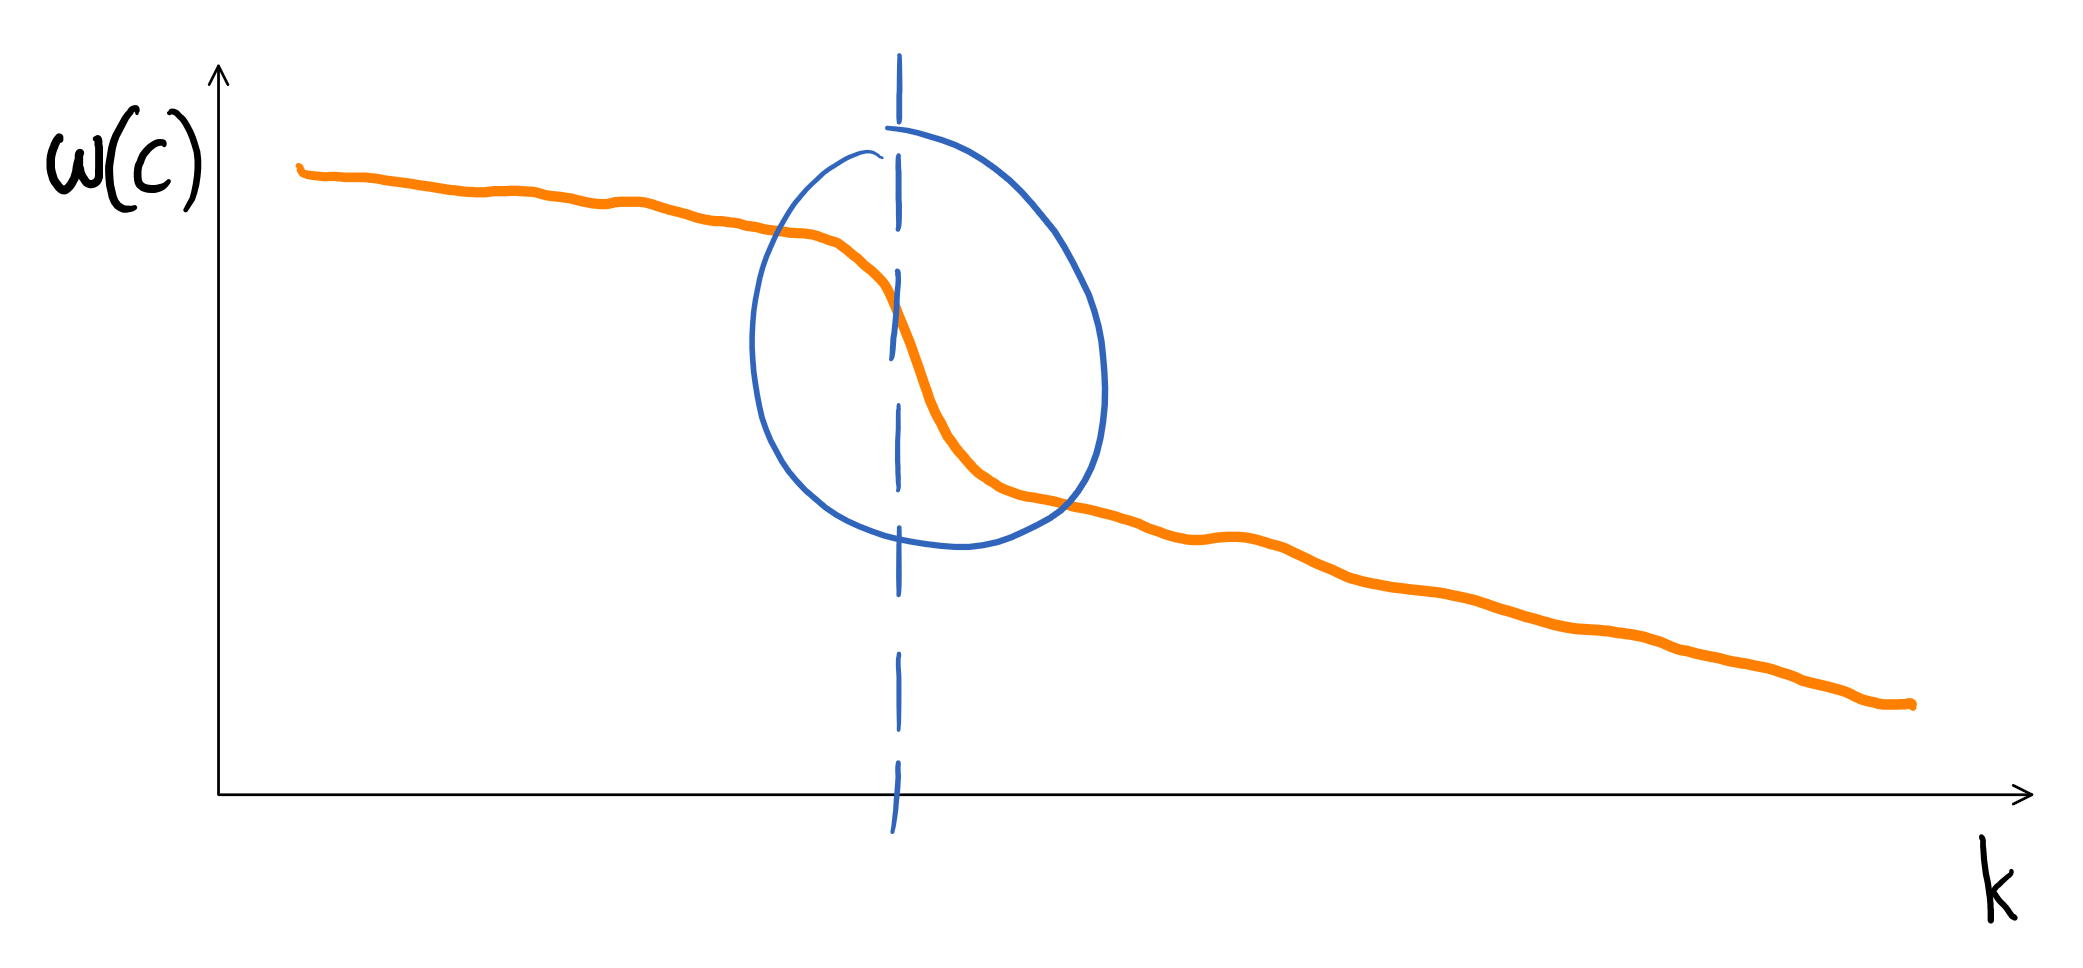
\includegraphics[width=0.8\textwidth]{07-rate-of-change}
% \end{figure}
%
% \subparagraph{Approach 2:} Let $w'(c)$ be a metric on a uniform distribution of samples. Relate change of $w(c)$ to change of $w'(c)$. Proposed in TEoSL.
%
% \begin{figure}[H]
% 	\centering
% 	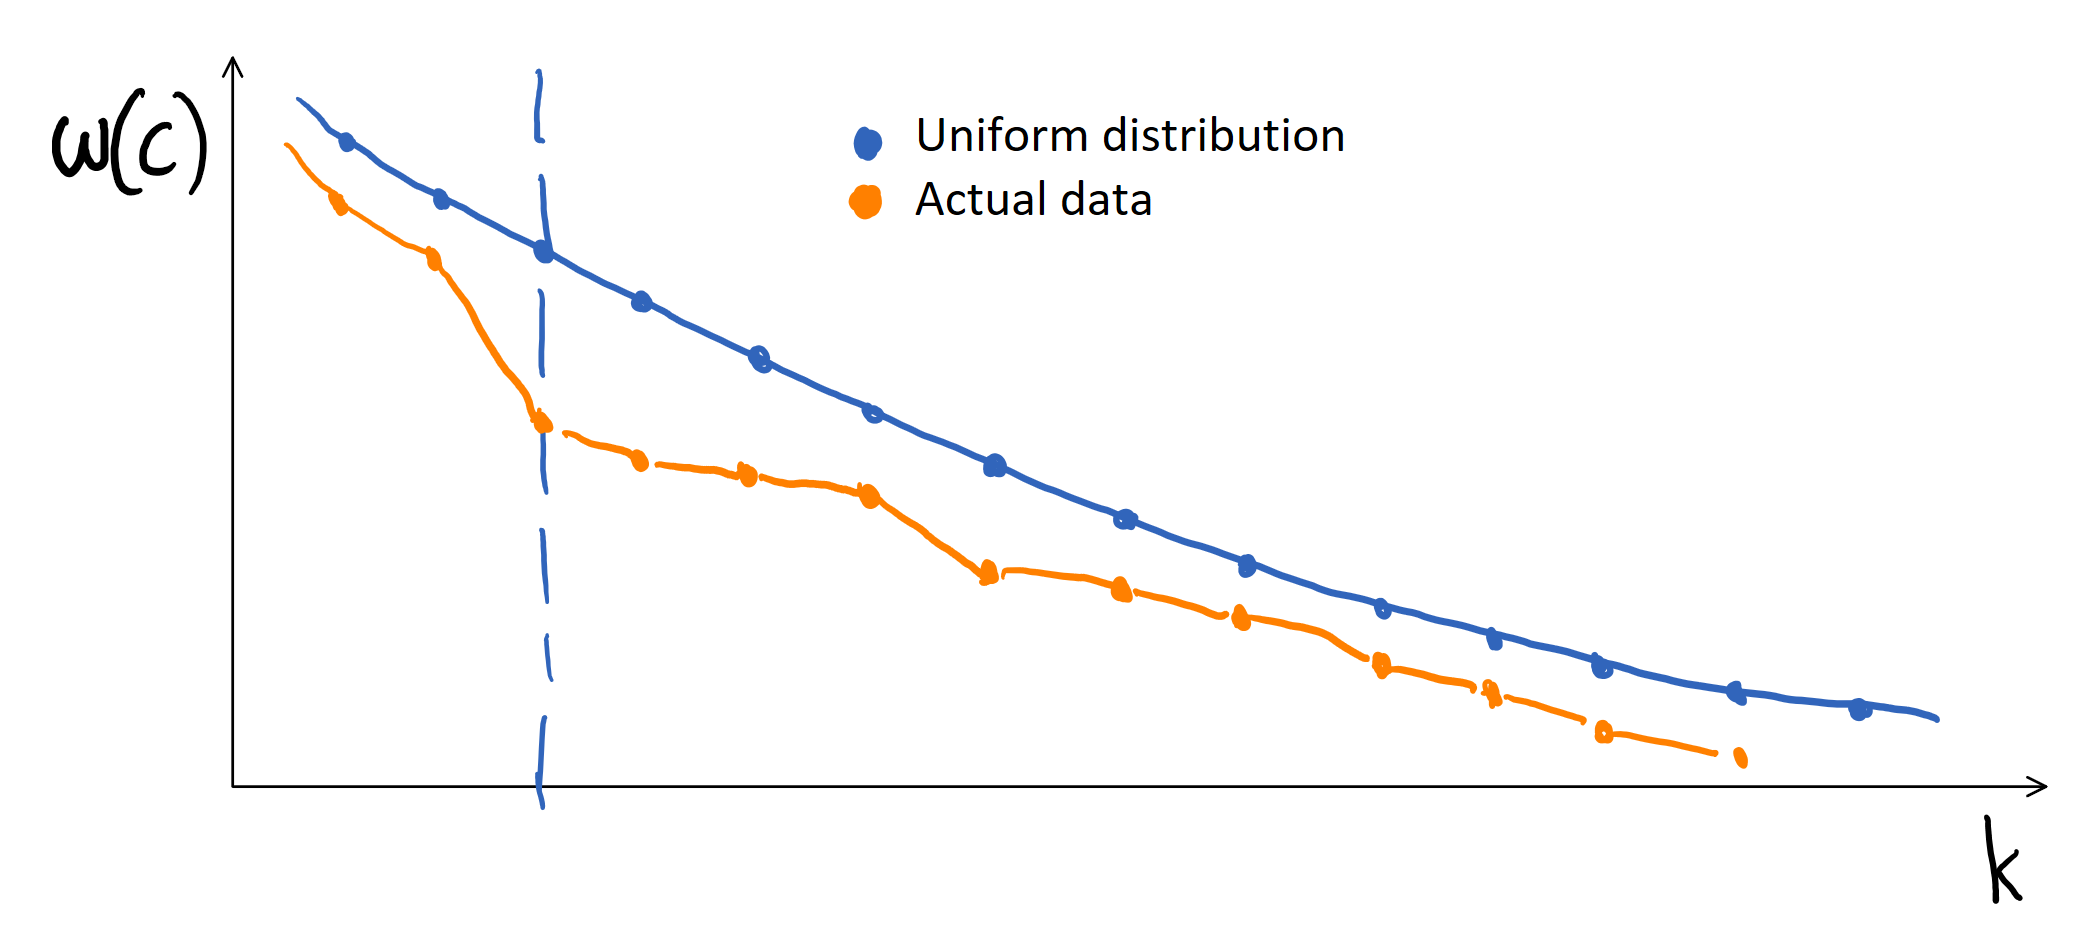
\includegraphics[width=0.8\textwidth]{08-w_c-vs-w_prime_c}
% \end{figure}
